\documentclass[10pt,twocolumn]{article}
\usepackage[T1]{fontenc}
\usepackage[utf8]{inputenc}
\usepackage{lmodern}
\usepackage[a4paper,margin=1.7cm,columnsep=0.65cm]{geometry}
\usepackage{amsmath,amssymb}
\usepackage{booktabs}
\usepackage{graphicx}
\usepackage{xcolor}
\usepackage{microtype}
\usepackage{tikz}
\usetikzlibrary{arrows.meta,positioning}
\usepackage[hidelinks]{hyperref}
\usepackage{url}
\hypersetup{
  pdftitle={Routeur: Cost-Aware Multi-Task LLM Routing Under a 10 ms CPU Budget},
  pdfauthor={Antoine CONTES and Tamara Wodzyński}
}

\title{Routeur: Cost-Aware Multi-Task LLM Routing\\Under a 10 ms CPU Budget}
\author{Antoine CONTES \and Tamara Wodzyński}
\date{July 2026}

\begin{document}
\maketitle

\begin{abstract}
Large language model routing is a constrained decision problem: a router should
select the cheapest model that is sufficiently capable for each request, while
adding negligible latency. We present Routeur, an open-source multi-task router
that jointly predicts a five-level difficulty target, task, risk, and required
capabilities. Two compact BERT students are dynamically quantized to INT8 and
served with ONNX Runtime. The 4.4M-parameter economy profile reaches 49.15\%
exact and 92.68\% adjacent validation accuracy, with 1.58\% severe
under-routing and a routed-cost ratio of 1.036 relative to the labelled oracle.
The 11.3M-parameter accuracy profile reaches 51.23\% exact and 93.38\%
adjacent accuracy, with 1.32\% severe under-routing. On an Intel Xeon E5-1650
v3 server their p95 decision latencies are 1.61 and 3.62 ms. We also describe a
critical limitation: under-routing and over-routing below 0.1\% would require at
least 99.8\% exact accuracy, which cannot be supported by the subjective and
boundary-noisy labels in the present corpus. Our evaluation therefore emphasizes
measured cost-quality Pareto points and explicit failure rates rather than an
unverifiable near-perfect claim.
\end{abstract}

\section{Introduction}
Routing every request to the most capable model wastes money and energy, while
routing every request to a small model degrades quality. Prior work has framed
this problem through preference prediction, benchmark-derived supervision, and
learned model selection~\cite{routellm,routerbench}. The deployment constraint is
often overlooked: if the router is slow or expensive, it consumes the benefit it
is intended to create.

Routeur targets a strict p95 CPU decision latency below 10 ms. The system makes
one semantic encoder pass, predicts four related targets, and applies a
cost-aware model policy. It exposes two production profiles instead of one
unqualified ``best'' model: an economy profile minimizes artifact size and cost,
whereas an accuracy profile accepts a modest cost increase for better routing.

This work contributes: (i) a compact multi-task architecture; (ii) a reproducible
data pipeline combining teacher labels, pairwise evidence, and public routing
datasets; (iii) INT8 CPU deployment with measured latency on two older Xeon
processors; (iv) explicit cost and asymmetric error metrics; and (v) an honest
analysis of the statistical ceiling imposed by the current labels.

\section{Problem Formulation}
For prompt $x$, the router predicts a level $\hat y\in\{1,\ldots,5\}$ and then
selects a callable model $m$ from catalog $\mathcal M$. The labelled oracle level
$y$ is the cheapest tier believed to satisfy a quality threshold. Let $c(m)$ be
normalized inference cost and $q(m,x)$ denote suitability. The deployment goal is
approximately
\begin{equation}
 \min_{m\in\mathcal M} c(m) \quad
 \text{subject to } q(m,x)\geq q_{\min},\quad L_{95}<10\text{ ms}.
\end{equation}

For a single five-way decision, exact, under-, and over-routing partition the
sample space:
\begin{equation}
 P(\hat y=y)+P(\hat y<y)+P(\hat y>y)=1.
\end{equation}
Consequently, requiring both directional errors below 0.1\% implies exact
accuracy above 99.8\%. This identity is independent of model architecture. It is
therefore invalid to report all three targets without an oracle whose agreement
and stability support that precision.

We report exact accuracy, adjacent accuracy $P(|\hat y-y|\leq1)$, severe
under-routing $P(y-\hat y\geq2)$, task accuracy, cost ratio to the labelled
oracle, savings relative to always using level 5, and uncached single-request
latency.

\section{Data Construction}
The final training mixture contains 49,984 normalized unique prompts. It combines
four evidence types. First, teacher-labelled prompts provide difficulty, task,
risk, and capability targets. Second, pairwise model outcomes reduce dependence
on purely verbal difficulty judgments. Third, MMR Routing 20K contributes
multi-turn conversations with independently observed weak-versus-strong model
scores~\cite{mmr}. Fourth, targeted synthetic examples improve coverage of rare
tasks and high-stakes language.

Exact normalized prompt overlap is removed across partitions. The 1,585-example
teacher-gold split is used for checkpoint and profile selection, so we call it a
validation set rather than a test set. A 3,000-example disjoint MMR set is kept as
an external diagnostic. Its tier labels are derived from observed score gaps and
do not define the same oracle as teacher-gold data. TwinRouterBench and
CodeRouterBench are retained as additional distribution-shift diagnostics
~\cite{twin,coderouter}.

This distinction matters. Difficulty levels compress a continuous, model- and
policy-dependent trade-off into five bins. Adjacent tiers often represent nearly
identical prompts, and teacher confidence is not a reliable proxy for label
agreement. The corpus is useful for model selection but cannot certify a 99.8\%
exact router.

\section{Architecture}
Figure~\ref{fig:architecture} summarizes inference. WordPiece tokenization is
bounded to 128 tokens. A compact bidirectional Transformer produces a pooled
representation $h$. Four heads predict level, task, risk, and multi-label
capabilities:
\begin{align}
 p_y &= \mathrm{softmax}(W_y h+b_y),\\
 p_t &= \mathrm{softmax}(W_t h+b_t),\\
 p_r &= \mathrm{softmax}(W_r h+b_r),\\
 p_c &= \sigma(W_c h+b_c).
\end{align}
Training minimizes a weighted sum of cross-entropy losses and binary
cross-entropy for capabilities. Shared representation learning is useful because
task, risk, and capability requirements provide semantic supervision even when
the precise level boundary is noisy.

\begin{figure}[t]
\centering
\resizebox{\columnwidth}{!}{%
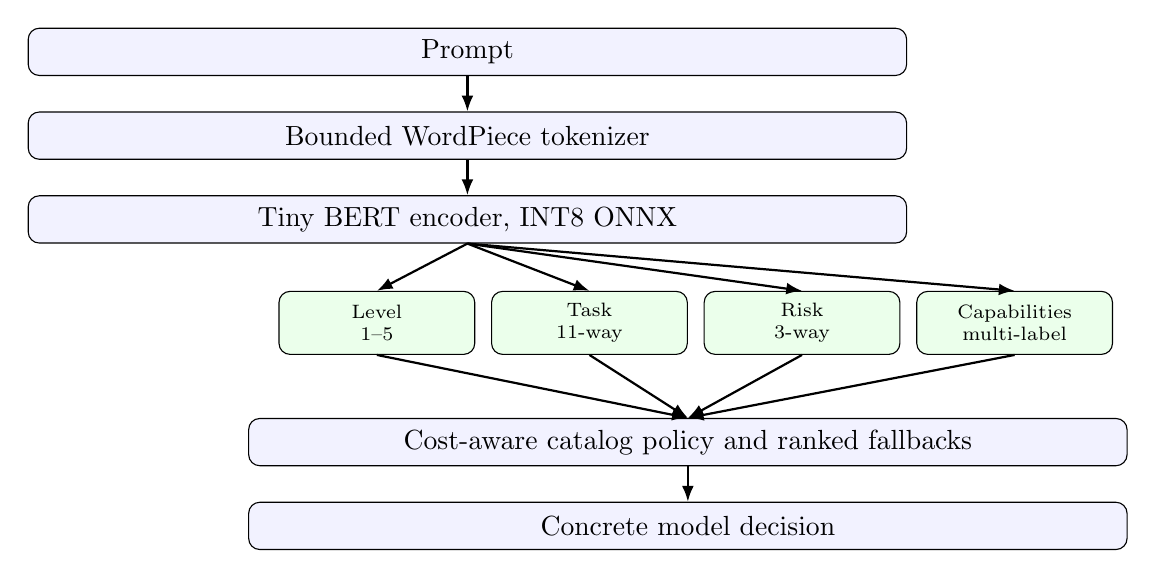
\begin{tikzpicture}[
  node distance=4.5mm,
  box/.style={draw,rounded corners,align=center,minimum width=0.92\columnwidth,minimum height=6mm,fill=blue!5},
  head/.style={draw,rounded corners,align=center,minimum width=0.205\columnwidth,minimum height=8mm,fill=green!8,font=\scriptsize},
  arr/.style={-{Latex[length=2mm]},thick}
]
\node[box] (prompt) {Prompt};
\node[box,below=of prompt] (tok) {Bounded WordPiece tokenizer};
\node[box,below=of tok] (enc) {Tiny BERT encoder, INT8 ONNX};
\node[head,below left=6mm and -1mm of enc.south] (lev) {Level\\1--5};
\node[head,right=2mm of lev] (task) {Task\\11-way};
\node[head,right=2mm of task] (risk) {Risk\\3-way};
\node[head,right=2mm of risk] (cap) {Capabilities\\multi-label};
\node[box,below=8mm of task.south east] (policy) {Cost-aware catalog policy and ranked fallbacks};
\node[box,below=of policy] (out) {Concrete model decision};
\draw[arr] (prompt)--(tok); \draw[arr] (tok)--(enc);
\foreach \x in {lev,task,risk,cap} \draw[arr] (enc.south)--(\x.north);
\foreach \x in {lev,task,risk,cap} \draw[arr] (\x.south)--(policy.north);
\draw[arr] (policy)--(out);
\end{tikzpicture}
}
\caption{Routeur inference architecture. The learned heads feed a catalog policy;
optional conservative guards can escalate high-stakes requests.}
\label{fig:architecture}
\end{figure}

The economy student uses the two-layer, 128-hidden, two-attention-head BERT Tiny
configuration~\cite{bert-tiny}; the accuracy student uses four layers, hidden
size 256, and four attention heads. A six-layer MiniLM candidate~\cite{minilm}
improved exact validation accuracy only marginally to 51.48\%, but its 12.52 ms
local p95 violated the deployment constraint and it was rejected.

\section{Training and Compression}
Training runs on an ephemeral H100 GPU using mixed precision, gradient clipping,
best-checkpoint selection, and a persistent artifact volume. No GPU container is
kept warm after the run. The two-layer model is trained for eight epochs; the
four-layer model for six. The encoder and all heads are exported together to
ONNX opset 17.

Dynamic signed INT8 quantization is applied to matrix multiplications. Dynamic
quantization is a natural CPU choice for Transformer weights and activations
whose ranges are computed at runtime~\cite{onnx-quant}. Per-channel weights and
reduced ranges are used for compatibility with older AVX2 CPUs. ONNX Runtime is
configured with one intra-op and one inter-op thread to reduce tail-latency
variance. The resulting artifacts, including tokenizers, are approximately 5 MB
and 12 MB.

An earlier hashed n-gram linear router is preserved as a reproducible baseline.
An ensemble with the semantic model increased validation accuracy, but the gain
did not persist on a held-out calibration partition; it was not promoted.

\section{Cost-Aware Policy}
The learned level is an internal compatibility signal rather than the final
product decision. The policy ranks callable catalog entries using tier fit, task
probabilities, required capability coverage, safety, public quality priors,
relative price, and provider-diverse fallbacks. Let $s(m,x)$ be the weighted
suitability score. A simplified view is
\begin{equation}
 m^*=\arg\max_{m\in\mathcal M}
 \left[s(m,x)-\lambda_c\widetilde c(m)-\lambda_o d(m,\hat y)\right],
\end{equation}
where $\widetilde c$ is normalized price and $d$ penalizes tier mismatch. Catalog
shortlists avoid scanning every model for every request.

The default profiles rely on learned risk, safety, and capability heads. Two
optional guard modes are available. A model-confirmed guard requires at least two
learned high-risk signals before escalation. A lexical guard escalates any
matched high-stakes phrase. The latter is intentionally conservative but caused
substantial false-positive level-5 routing on validation data, so it is not the
cost-optimized default.

\section{Experimental Results}
All latency measurements use 20 warm-ups and 1,000 unique prompts, which bypass
the in-process LRU cache. Runs are sequential and use one ONNX Runtime thread.
Table~\ref{tab:results} reports the teacher-gold validation results. Exact values
are available in each artifact's \texttt{evaluation.json}.

\begin{table}[t]
\centering
\caption{Validation cost-quality results. Lower is better for severe
under-routing and cost ratio; higher is better otherwise.}
\label{tab:results}
\small
\begin{tabular}{lrrr}
\toprule
Metric & Linear & Economy & Accuracy \\
\midrule
Exact accuracy (\%) & 48.39 & 49.15 & \textbf{51.23} \\
Adjacent accuracy (\%) & 91.92 & 92.68 & \textbf{93.38} \\
Severe under-route (\%) & 2.78 & 1.58 & \textbf{1.32} \\
Task accuracy (\%) & 59.50 & 58.30 & \textbf{61.83} \\
Savings vs level 5 (\%) & 88.98 & \textbf{89.07} & 88.10 \\
Cost/oracle & -- & \textbf{1.036} & 1.128 \\
Artifact (MB) & 52 & \textbf{5} & 12 \\
\bottomrule
\end{tabular}
\end{table}

The economy model is the strongest cost point: it is smaller than the linear
baseline, improves exact and adjacent accuracy, nearly halves severe
under-routing, and spends only 3.6\% above the labelled oracle. The accuracy
profile improves exact accuracy by another 2.08 percentage points and lowers
severe under-routing, but spends 12.8\% above the oracle. Thus neither profile
dominates the other.

\begin{table}[t]
\centering
\caption{Uncached single-prompt CPU p95 latency in milliseconds.}
\label{tab:latency}
\small
\begin{tabular}{lrrr}
\toprule
Machine & Economy & Accuracy & 10 ms SLO \\
\midrule
Xeon E3-1271 v3 & 2.84 & 4.76 & pass \\
Xeon E5-1650 v3 & 1.61 & 3.62 & pass \\
\bottomrule
\end{tabular}
\end{table}

Both profiles satisfy the target with substantial margin
(Table~\ref{tab:latency}). The rejected six-layer candidate demonstrates why
architecture selection must include measured tail latency rather than parameter
count or average time alone.

On the disjoint MMR diagnostic, economy and accuracy exact scores are 33.00\% and
37.47\%, while severe under-routing is 39.27\% and 34.33\%. These poor absolute
rates reveal a major oracle shift: MMR levels encode observed performance gaps
between particular weak and strong models, whereas teacher-gold levels encode a
general difficulty judgment. We report these results because they prevent a
misleading in-distribution interpretation. They are evidence that future work
must train and evaluate against the same operational quality threshold and model
catalog.

\section{Limitations and Threats to Validity}
The principal limitation is label validity. Five discrete tiers are not natural
ground truth, and a prompt's cheapest sufficient model changes with the model
catalog, price, decoding settings, and quality threshold. The validation set was
used for checkpoint selection. It measures model-selection quality, not a final
unbiased generalization estimate.

Second, cost figures use a normalized policy snapshot rather than audited bills
from a randomized production trial. Prompt and completion length distributions
can change the realized savings. Third, latency is measured on two x86 CPUs and
does not cover all runtime versions, contention levels, or ARM deployments.
Fourth, disabling a hard lexical guard reduces false-positive escalation and cost
but makes safety depend on learned heads. High-stakes deployments should select a
conservative mode and measure its quality-cost consequences on their own traffic.

The near-100\% objective should be revisited only after constructing a stable
oracle. A suitable protocol would run every candidate model on each prompt,
score outputs with multiple independent judges and human adjudication near tier
boundaries, repeat ambiguous trials, and reserve a never-touched temporal test
set. Selective routing with abstention could then guarantee low directional error
on the accepted subset, at the cost of escalating uncertain requests.

\section{Reproducibility}
The public repository contains data builders, training code, model cards, ONNX
export and quantization, both production artifacts, a latency gate, evaluation
metrics, and continuous integration. Raw third-party datasets are downloaded from
their publishers to preserve licenses and provenance. The command-line interface
can select either profile and can override the safety guard mode. Tests validate
calibration, routing, batching, policy behavior, and serialization.

\section{Conclusion}
Routeur demonstrates that semantic multi-task routing can fit comfortably inside
a 10 ms CPU budget without a large runtime artifact. The economy profile offers
the best measured cost point, while the four-layer profile offers the best
in-distribution accuracy and severe-under-routing result. More importantly, the
experiments expose the gap between optimizing a noisy five-tier teacher label and
measuring true cheapest-sufficient-model decisions. Progress toward near-perfect
routing now depends more on a stable, production-aligned oracle than on increasing
encoder size.

\begin{thebibliography}{9}
\bibitem{routellm}
Ong et al. RouteLLM: Learning to Route LLMs with Preference Data. arXiv:2406.18665, 2024.

\bibitem{routerbench}
Hu et al. RouterBench: A Benchmark for Multi-LLM Routing System. arXiv:2403.12031, 2024.

\bibitem{minilm}
Wang et al. MiniLM: Deep Self-Attention Distillation for Task-Agnostic Compression of Pre-Trained Transformers. arXiv:2002.10957, 2020.

\bibitem{bert-tiny}
Turc et al. Well-Read Students Learn Better: On the Importance of Pre-training Compact Models. arXiv:1908.08962, 2019.

\bibitem{mmr}
J. Xue. MMR Routing 20K dataset. Hugging Face, Apache-2.0. \url{https://huggingface.co/datasets/JiaqiXue/mmr-routing-20k}

\bibitem{twin}
Amorph. TwinRouterBench dataset. Hugging Face, Apache-2.0. \url{https://huggingface.co/datasets/Amorph/TwinRouterBench}

\bibitem{coderouter}
Lance1573. CodeRouterBench dataset. Hugging Face, MIT. \url{https://huggingface.co/datasets/Lance1573/CodeRouterBench}

\bibitem{onnx-quant}
ONNX Runtime. Quantize ONNX models. \url{https://onnxruntime.ai/docs/performance/model-optimizations/quantization.html}
\end{thebibliography}

\end{document}
